\subsection{Power system of Railway Transportation System}

\begin{frame}{Railway Transportation System}{Overview of Existing European Railway Power Systems}
	\begin{block}{\textbf{Overview of Existing European Railway Power Systems}}
	%	Back to the 19th century, the steam turbine was the main propulsion system for the trains. Later on, electric and diesel propulsion systems were adopted. In recent years occurred a massive introduction of power converters based on \ac{IGBT}, which allowed an increase of energy efficiency (allowing, for example, regenerative breaking and reduction of power losses in traction motors).
		
	%	Due to this evolution, different topologies of the railway system exists nowadays. In table \ref{tab:31.t1}, different catenary topologies are visible which results in different power systems for \ac{RTS}.
		
		

			% Table generated by Excel2LaTeX from sheet 'Sheet1'
\begin{table}[htbp]
	\centering
	\tiny
	\caption{Catenary topology and vehicle characteristics of different railway vehicles. \cite{abad2016}.}
	\begin{tabular}{|c|p{10.145em}p{10.355em}|cc|}
		\cmidrule{2-5}    \multicolumn{1}{c|}{} & \multicolumn{2}{c|}{\textbf{Catenary topology}} & \multicolumn{2}{c|}{\textbf{Vehicle characteristics}} \\
		\cmidrule{2-5}    \multicolumn{1}{c|}{} & \multicolumn{1}{c}{\textbf{DC supply}} & \multicolumn{1}{c|}{\textbf{AC supply}} & \textbf{Power} & \textbf{Top speed} \\
		\midrule
		\textbf{Tram} & 600V DC, 750V DC, 900V DC & \multicolumn{1}{c|}{-}     & 150–300kW & 50–70km/h \\
		\midrule
		\textbf{Metro} & 750V DC, 1500V DC & \multicolumn{1}{c|}{-}     & 350kW–1MW & 80km/h \\
		\midrule
		\textbf{Train} & 750V DC, 1500V DC, 3000V DC & 15kV AC (16.7Hz) and 25kV AC (50Hz) & 200kW–8MW & 120–350km/h \\
		\midrule
		\textbf{Locomotive} & 750V DC, 1500V DC, 3000V DC & 15kV AC (16.7Hz) and 25kV AC (50Hz) & 500kW–8MW & 100–200km/h \\
		\bottomrule
	\end{tabular}%
	\label{tab:31.t1}%
\end{table}%


		
	\end{block}
\end{frame}
%%%%%%%%%%%%%%%%%%%%%%%%%%%%%%%%%%%%%%%%%%%%%%%%%%%%%%%%%%%%%%%%%%%%%%%%%%%%%%%%%%%%%

\begin{frame}{Railway Transportation System}{Overview of Existing European Railway Power Systems}
%\begin{block}{\textbf{Overview of Existing European Railway Power Systems}}


\begin{figure}[h!]
	\centering
	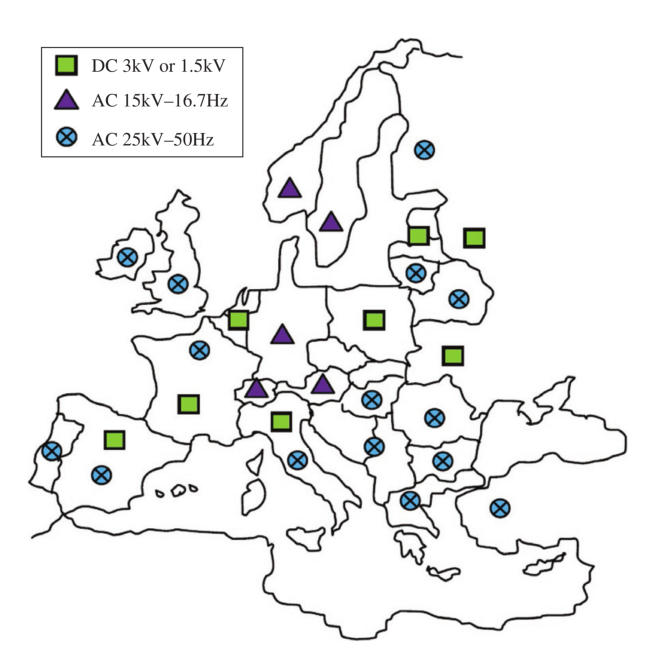
\includegraphics[width=0.4\textwidth,keepaspectratio]{figures/31.PowerS/abad2016}
	\caption{Railway main-line power supply systems in Europe. \cite{abad2016}.}
	\label{fig:abad2016}
\end{figure}
	
	
%\end{block}
\end{frame}
%%%%%%%%%%%%%%%%%%%%%%%%%%%%%%%%%%%%%%%%%%%%%%%%%%%%%%%%%%%%%%%%%%%%%%%%%%%%%%%%%%%%%

\subsection{Railway Power Supply System}


\begin{frame}{Railway Transportation System}{Overview of Existing European Railway Power Systems}
	\begin{minipage}[t]{0.48\linewidth}
	%\begin{itemize}
	%	\item \ac{DC} supply system architecture	
	%\end{itemize}
	
	\begin{figure}[ht!]
		\centering
		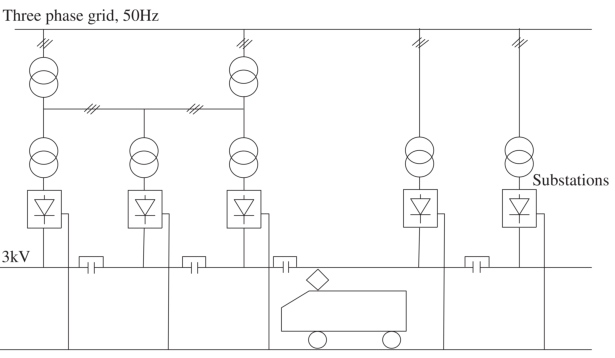
\includegraphics[width=0.7\textwidth,keepaspectratio]{figures/31.PowerS/abad2016f}
		\caption{\ac{DC} supply system architecture. \cite{abad2016}.}
	\end{figure}
\end{minipage}\hfill
\begin{minipage}[t]{0.48\linewidth}
	%\begin{itemize}
	%	\item  50 Hz 25 kV supply system.
	
	%\end{itemize}
	
	\begin{figure}[ht!]
		\centering
		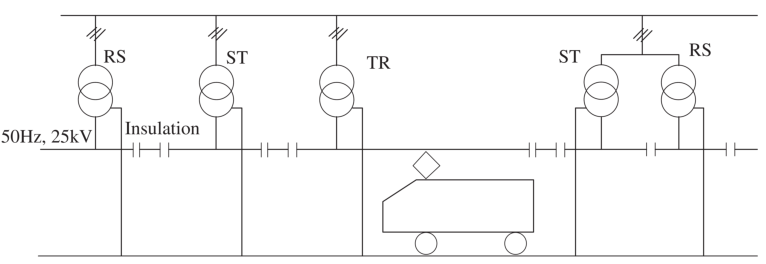
\includegraphics[width=\textwidth,keepaspectratio]{figures/31.PowerS/abad2016d}
		\caption{50 Hz 25 kV supply system. \cite{abad2016}.}
	\end{figure}

	\begin{figure}[ht!]
	\centering
	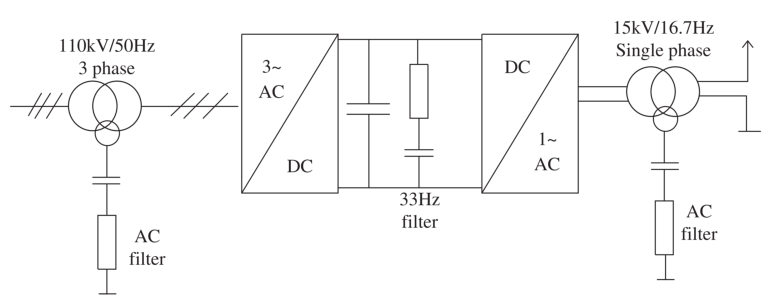
\includegraphics[width=\textwidth,keepaspectratio]{figures/31.PowerS/abad2016e}
	\caption{16.7 Hz 15 kV supply system. \cite{abad2016}.}
\end{figure}
	
\end{minipage}

\end{frame}
%%%%%%%%%%%%%%%%%%%%%%%%%%%%%%%%%%%%%%%%%%%%%%%%%%%%%%%%%%%%%%%%%%%%%%%%%%%%%%%%%%%%%
